

\subsection{Richtlinien von 'Human-Centered Autonomous Vehicles(HCAV)' \cite{b5} }
Dieses Kapitel enthält eine Aufführung der Richtlinien nach Lex Fridman\cite{b6}. Die Quelle selber ist auf Englisch verfasst, weshalb Zitate von mir übersetzt werden. Die Idee hinter diesen Richtlinien ist, eine Sammlung von Elementen zu definieren die für das Entwickeln und Bauen Autonomer Fahrzeuge stetig in Betracht gezogen werden.\\
Dabei sind Drei weit verbreitete Gedanken bezüglich autonomer Fahrzeuge:
\begin{itemize}
	\item[1. ]Selbstständiges Fahren ist einfach Machbar.\cite{b7,b8,b9}
	\item[2. ]Menschen sind schlechte Autofahrer.\cite{b10,b11}
	\item[3. ]Mensch und Maschine passen nicht zueinander.\cite{b12,b13}
\end{itemize}
Fridman sagt, dass diese Drei Punkte jedoch eher dem jeweiligen Gegenteil entsprechen und stellt die 7 Richtlinien das Mensch-zentrierten Designs auf. Für eine detailliertere Beschreibung dieser verweise ich auch das Paper(siehe oben).\\

\textbf{Richtlinie 1: Geteilte/Transparente Autonomie}\\
Der Fahrer soll während das Auto alleine fährt mehr in die Fahrt integriert werden. Grund hierfür ist, dass Teilautonome Fahrzeuge immer wieder von Fahrern übernommen werden müssen und diese somit die wichtigsten Informationen der Situation verständlich aufnehmen können müssen. Fridman führt dabei eine Tabelle auf in der ersichtlich wird, welche System wie gut sein müssen für die Stufen 4 \& 5 autonomen Fahrens. \cite{b14}
\begin{figure}[!h]
	\centering
	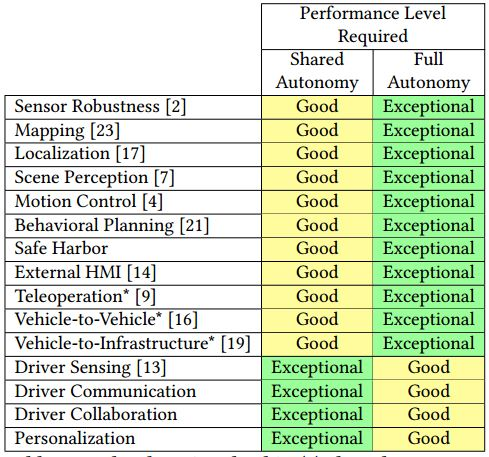
\includegraphics[width=0.45\columnwidth]{pictures/reqTableLexFridman.jpg}
	\caption{Erforderliche Technologien und ihr 'Level' in Stufe 4 \& 5 Fahrzeugen.
		Hier muss ich die Tabelle nochmal selber machen und Quellen aktuell halten.}
	\label{img:fridman1}
\end{figure}

\textbf{Richtlinie 2: Von aufgenommenen Daten lernen} \\
Jede in der obigen Tabelle aufgeführte Technologie soll datengesteuert sein und sich selber iterativ mit Hilfe der erfassten Daten selber verbessern können. Durch gutes Mapping der Features innerhalb eines Autos zueinander ist es möglich, hiervon Datensets für betreutes Lernen zur kreieren. \label{sec:rl2}Dank dieses sich immer wiederholenden Prozesses können Autos in der Zukunft selber von aufgenommenen Daten lernen und sich somit besser dem Fahrer anpassen.\\

\textbf{Richtlinie 3: Fahrerbeobachtung}\\
Bis auf wenige Ausnahmen nutzt kaum ein Unternehmen interne Kameras zum Deuten von Nutzergesten und Beobachten der Fahreraufmerksamkeit. Im Prototypen des HCAV Programms wurden die eben aufgeführten Aspekte von Innenkameras aufgezeichnet und gedeutet. Dadurch kann das Auto mit dem Fahrer kommunizieren wenn es dies als notwendig empfindet. Zu wissen ob der Fahrer abgelenkt, gestresst, müde oder sonstiges ist steigere nicht nur die Fahrsicherheit enorm, sondern unterstützt auch Richtlinie 1 stark.\\

\textbf{Richtlinie 4: Geteilte Wahrnehmungskontrolle}\\
Diese Richtlinie definiert das Ziel, den Status der Systemfähigkeiten und -einschränkungen dem Fahrer stetig zur Verfügung zu stellen. Hierdurch kann dieser das Verhalten des Autos mitverfolgen und Up-to-date mit der Auto-Umwelt bleiben wodurch die Sicherheit bei einer Übernahme des Fahrers gesteigert wird.\\
Auch hier wird stetig von aufgenommenen Daten gelernt, um so bspw. die Lenkart des Fahrers zu imitieren. \textit{\hyperref[sec:rl2]{siehe: Richtlinie 2}}
\\

\textbf{Richtlinie 5: Fahrzeug Personalisierung}\\
Das Auto soll jeden Fahrer einzeln detailliert kennenlernen und sich an diese anpassen wenn sie das Auto betreten. Von Beginn an soll das Auto verschiedene Aspekte des Fahrers kennenlernen(Körpersprache, Mimik, Gestik, Sprachgebrauch,Fahrweise, etc.). Somit ist nach bereits kurzer Zeit jede Konfiguration für Fahrer einzigartig und somit höchst personalisiert.
\\

\textbf{Richtlinie 6: Unvollkommenes Design}\\
Ein Auto soll nicht zur Perfektion streben, sondern Fehler/Schwierige Situationen geeignet Kommunizieren. Durch das Erkennen solcher Situationen gewinnt das Auto nach Auswertung einen hohen Mehrwert. Wichtig ist auch, dass der Fahrer über diese informiert wird. Die bis jetzt beste Art dies zu tun, ist dem Fahrer die Umwelt aus Sicht des Autos zu zeigen(Fig. 2).
\begin{figure}[H]
	\centering
	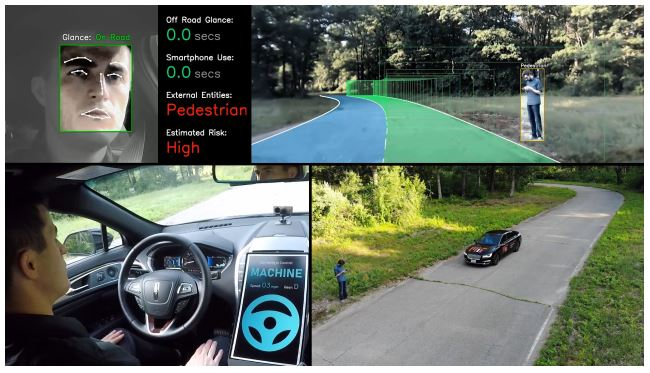
\includegraphics[width=0.734\columnwidth]{pictures/CarView.jpg}
	\caption{Erforderliche Technologien und ihr 'Level' in Stufe 4 \& 5 Fahrzeugen.
		Hier muss ich die Tabelle nochmal selber machen und Quellen aktuell halten.}
	\label{img:CarView}
\end{figure}

\textbf{Richtlinie 7: System-Level Experience}\\
Da weder Fahrzeuge noch Menschen perfekt sind, müssen die Fehler ausgewertet werden um zu Versuchen, daraus zu lernen. Dies soll nicht nur Fahrsicherheitsaspekte betreffen, sondern auch Fehler die im Rahmen Vergnügungsfeatures aufgetreten sind.